% Created 2025-02-05 Wed 10:53
% Intended LaTeX compiler: pdflatex
\documentclass[11pt]{article}
\usepackage[latin1]{inputenc}
\usepackage[T1]{fontenc}
\usepackage{graphicx}
\usepackage{longtable}
\usepackage{wrapfig}
\usepackage{rotating}
\usepackage[normalem]{ulem}
\usepackage{amsmath}
\usepackage{amssymb}
\usepackage{capt-of}
\usepackage{hyperref}
\date{\today}
\title{Creating a Cyber Range (JIA)}
\hypersetup{
 pdfauthor={},
 pdftitle={Creating a Cyber Range (JIA)},
 pdfkeywords={},
 pdfsubject={},
 pdfcreator={Emacs 29.4 (Org mode 9.6.15)}, 
 pdflang={English}}
\begin{document}

\maketitle
\tableofcontents

\section{Goal}
\label{sec:org0dacc84}
The goal of this exercise is to create a cyber range.
\subsection{Topology}
\label{sec:org410d5ba}
\begin{center}
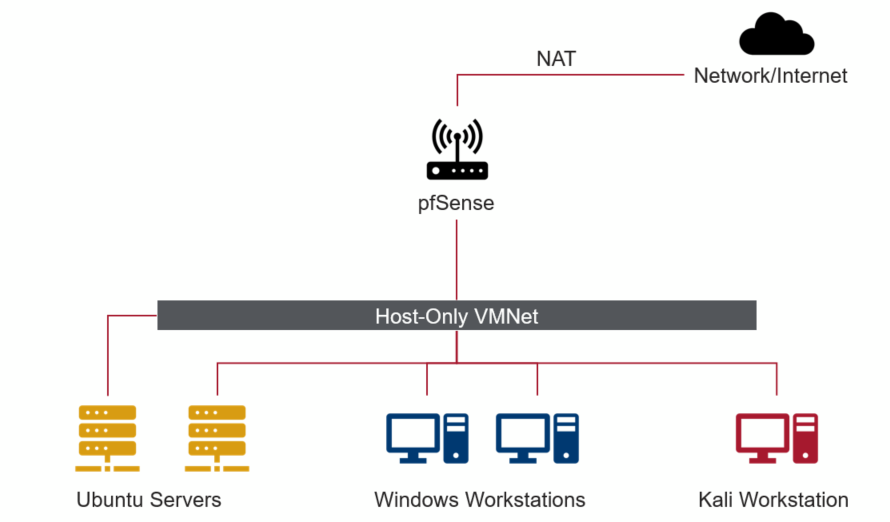
\includegraphics[width=.9\linewidth]{./img/topology.png}
\end{center}
\section{Virtual machine installs}
\label{sec:org725aadd}
\subsection{Ubuntu-Server-01}
\label{sec:org7da871f}
\subsubsection{VM Specs}
\label{sec:org3629aaf}
\begin{itemize}
\item 20GB - HDD in single file
\item NIC:
\begin{itemize}
\item On setup: NAT
\item After setup: Host-Only
\end{itemize}
\end{itemize}
\subsubsection{Install}
\label{sec:orgf8850c4}
DHCP bound 192.168.246.135/24
Set up sda with LVM taking up the whole drive apart from /boot (1.771G)
\begin{center}
\begin{tabular}{lll}
Part & Size & Format\\[0pt]
\hline
/boot & 1.771G & ext4\\[0pt]
free & 8.22G & -\\[0pt]
\end{tabular}
\end{center}
\begin{enumerate}
\item Username
\label{sec:org6d77f20}
user:user
\item Software
\label{sec:orged7f996}
OpenSSH server
No other software
\end{enumerate}
\subsection{pfsense}
\label{sec:org10c02e0}
\subsubsection{VM Specs}
\label{sec:org8ee7017}
\begin{itemize}
\item 20GB -  HDD in one file
\item NIC:
\begin{itemize}
\item On Setup: NAT
\item After setup:
\begin{itemize}
\item NIC 1: NAT
\begin{itemize}
\item MAC:
\end{itemize}
\item NIC 2: Host-Only
\begin{itemize}
\item MAC:
\end{itemize}
\end{itemize}
\end{itemize}
\end{itemize}
\subsubsection{Install}
\label{sec:org2294b6e}
ZFS guided install single "striped" install
\subsection{Ubuntu-Server-02}
\label{sec:org645ab7f}
Linked clone of \ref{sec:org7da871f}
\subsubsection{Username}
\label{sec:org1dd6273}
user:user
\subsection{Kali-Blue}
\label{sec:org6fa65d3}
Copy the extracted virtual machine into Desktop/VMs where the rest of the VMs created so far are and open the kali.vmx file.
\subsubsection{Username}
\label{sec:orga01ccca}
kali:kali
\subsection{Kali-Purple}
\label{sec:org71ee4ba}
\subsubsection{VM specs}
\label{sec:org0214a3c}
\begin{itemize}
\item 60GB - HDD in single file
\item NIC:
\begin{itemize}
\item On setup: NAT
\item After setup: Host-Only
\end{itemize}
\end{itemize}
\subsubsection{Username}
\label{sec:org38818b7}
kali:kali
\subsubsection{Install}
\label{sec:orgb23c693}
\begin{center}
\begin{tabular}{lll}
Part & Size & Format\\[0pt]
\hline
swap & 3.3G & swap\\[0pt]
\end{tabular}
\end{center}
\begin{enumerate}
\item Extra software
\label{sec:org0ca87ac}
\begin{itemize}
\item Desktop
\begin{itemize}
\item XFCE
\end{itemize}
\item Defensive Tools
\begin{itemize}
\item Identify
\item Protect
\item Detect
\item Respond
\item Recover
\end{itemize}
\end{itemize}
\end{enumerate}
\subsection{Win10-V}
\label{sec:org98b50f6}
Imported from provided MSEdge-Win10-VMware.ovf file
\subsubsection{Username}
\label{sec:org11e0769}
IEUser:Passw0rd!
\subsection{Win10-H}
\label{sec:orgb8481a0}
Cloned from \ref{sec:org98b50f6} as a full clone
\subsubsection{Username}
\label{sec:orgcbdcb48}
IEUser:Passw0rd!

\section{Excursus on exporting}
\label{sec:org3d56cae}
The lab has an exercise in exporting and importing VMs this has been skipped for brevities sake
\section{Virtual Network}
\label{sec:org4cacf31}
\end{document}
